\chapter{Attention Variants and Mechanisms}
\label{chap:attention_variants}

\section*{Chapter Overview}

Beyond standard scaled dot-product attention, numerous variants have been developed for specific use cases and improved efficiency. This chapter explores cross-attention for encoder-decoder models, soft vs hard attention, attention with relative position representations, and practical considerations for implementing attention mechanisms.

\subsection*{Learning Objectives}

\begin{enumerate}
    \item Distinguish between self-attention and cross-attention
    \item Understand relative position representations
    \item Implement attention with different scoring functions
    \item Apply attention masking for various scenarios
    \item Understand attention dropout and layer normalization
    \item Visualize and interpret attention patterns
\end{enumerate}

\section{Cross-Attention}
\label{sec:cross_attention}

\begin{definition}[Cross-Attention]
\label{def:cross_attention}
In encoder-decoder architectures, decoder attends to encoder output via cross-attention:
\begin{align}
\mQ &= \mX_{\text{dec}} \mW^Q \quad \text{(queries from decoder)} \\
\mK &= \mX_{\text{enc}} \mW^K \quad \text{(keys from encoder)} \\
\mV &= \mX_{\text{enc}} \mW^V \quad \text{(values from encoder)} \\
\text{CrossAttn}(\mX_{\text{dec}}, \mX_{\text{enc}}) &= \text{softmax}\left(\frac{\mQ \mK\transpose}{\sqrt{d_k}}\right) \mV
\end{align}
\end{definition}

\textbf{Dimensions:}

\begin{mermaid}[Cross-Attention vs Self-Attention Data Flow]
graph LR
    subgraph SelfAttn["Self-Attention"]
        SX["X in R^n x d"] --> SQ["Q from X"]
        SX --> SK["K from X"]
        SX --> SV["V from X"]
        SWQ["W_Q"] --> SQ
        SWK["W_K"] --> SK
        SWV["W_V"] --> SV
        SQ --> SOUT["Output in R^n x d\n Memory: O(n^2)"]
        SK --> SOUT
        SV --> SOUT
    end

    subgraph CrossAttn["Cross-Attention"]
        DX["Decoder X_dec\n in R^m x d"] --> CQ["Q = X_dec*W_Q\n in R^m x d_k"]
        CWQ["W_Q\n in R^d x d_k"] --> CQ
        EX["Encoder X_enc\n in R^n x d"] --> CK["K in R^n x d_k"]
        EX --> CV["V in R^n x d_v"]
        CWK["W_K\n in R^d x d_k"] --> CK
        CWV["W_V\n in R^d x d_v"] --> CV
        CQ --> COUT["Output in R^m x d_v\n Memory: O(m*n)"]
        CK --> COUT
        CV --> COUT
    end

    style SX fill:#e8f5e9,stroke:#4caf50,color:#000
    style DX fill:#e3f2fd,stroke:#2196f3,color:#000
    style EX fill:#e8f5e9,stroke:#4caf50,color:#000
    style SWQ fill:#fff3e0,stroke:#ff9800,color:#000
    style SWK fill:#fff3e0,stroke:#ff9800,color:#000
    style SWV fill:#fff3e0,stroke:#ff9800,color:#000
    style CWQ fill:#fff3e0,stroke:#ff9800,color:#000
    style CWK fill:#fff3e0,stroke:#ff9800,color:#000
    style CWV fill:#fff3e0,stroke:#ff9800,color:#000
    style COUT fill:#f3e5f5,stroke:#9c27b0,color:#000
\end{mermaid}

\begin{itemize}
    \item Decoder input: $\mX_{\text{dec}} \in \R^{m \times d}$ ($m$ decoder positions)
    \item Encoder output: $\mX_{\text{enc}} \in \R^{n \times d}$ ($n$ encoder positions)
    \item Attention matrix: $\mA \in \R^{m \times n}$ (decoder $\times$ encoder)
    \item Output: $\R^{m \times d_v}$ (same decoder length)
\end{itemize}

\begin{example}[Machine Translation Cross-Attention]
\label{ex:translation_cross_attention}
English source: "The cat sat" (3 tokens encoded to $\mX_{\text{enc}} \in \R^{3 \times 512}$)

French target: "Le chat" (2 tokens so far, $\mX_{\text{dec}} \in \R^{2 \times 512}$)

Cross-attention computes:
\begin{equation}
\mA = \begin{bmatrix}
\alpha_{1,1} & \alpha_{1,2} & \alpha_{1,3} \\
\alpha_{2,1} & \alpha_{2,2} & \alpha_{2,3}
\end{bmatrix} \in \R^{2 \times 3}
\end{equation}

where $\alpha_{1,j}$ = attention from decoder position 1 ("Le") to encoder position $j$.

When generating "Le" (the), model should attend strongly to "The" in source.

When generating "chat" (cat), model should attend strongly to "cat" in source.
\end{example}

\subsection{Transformer Decoder Attention Layers}

A transformer decoder block contains \textbf{three} attention mechanisms:

\begin{enumerate}
    \item \textbf{Masked self-attention:} Decoder attends to previous decoder positions
    \begin{equation}
    \mQ = \mK = \mV = \mX_{\text{dec}} \quad \text{(with causal mask)}
    \end{equation}

    \item \textbf{Cross-attention:} Decoder attends to encoder output
    \begin{equation}
    \mQ = \mX_{\text{dec}}, \quad \mK = \mV = \mX_{\text{enc}}
    \end{equation}

    \item \textbf{Feed-forward:} Position-wise MLP (not attention)
\end{enumerate}

\begin{keypoint}
Encoder-only models (BERT) use only self-attention. Decoder-only models (GPT) use only masked self-attention. Encoder-decoder models (T5, BART) use all three mechanisms.
\end{keypoint}

\section{Relative Position Representations}
\label{sec:relative_position}

\textbf{Problem with absolute positions:} Model learns positions 0-512 during training. How to handle position 600 at inference?

\textbf{Solution:} Relative position representations—encode distance between positions, not absolute positions.

\subsection{Shaw et al. Relative Attention}

\begin{definition}[Relative Position Attention]
\label{def:relative_position_attention}
Modify attention scores to include relative position information:
\begin{equation}
e_{ij} = \frac{\vq_i\transpose \vk_j}{\sqrt{d_k}} + \vq_i\transpose \vr^{K}_{i-j}
\end{equation}
where $\vr^{K}_{i-j} \in \R^{d_k}$ encodes relative position $i-j$ (clipped to maximum distance).
\end{definition}

\textbf{Advantages:}
\begin{itemize}
    \item Generalize to longer sequences
    \item Model learns distance-based patterns
    \item More parameter efficient
\end{itemize}

\subsection{T5 Relative Position Bias}

T5 uses even simpler approach—add learned bias based on relative position:
\begin{equation}
\mA_{ij} = \text{softmax}\left(\frac{\mQ \mK\transpose}{\sqrt{d_k}} + \mB\right)_{ij}
\end{equation}
where $B_{ij}$ depends only on $|i-j|$ (bucketed by distance).

\section{Alternative Attention Scoring Functions}
\label{sec:scoring_functions}

Beyond the scaled dot-product used in transformers, several alternative scoring functions exist---additive (Bahdanau), multiplicative (Luong), and general bilinear forms---each with different trade-offs between expressiveness and computational efficiency. These are defined and compared in Chapter~\ref{chap:attention_fundamentals} (Section~7.3). In practice, scaled dot-product attention dominates in transformer architectures due to its hardware-efficient batched matrix multiplication and strong empirical performance.

\section{Attention Masking}
\label{sec:attention_masking}

\begin{figure}[h]
\centering
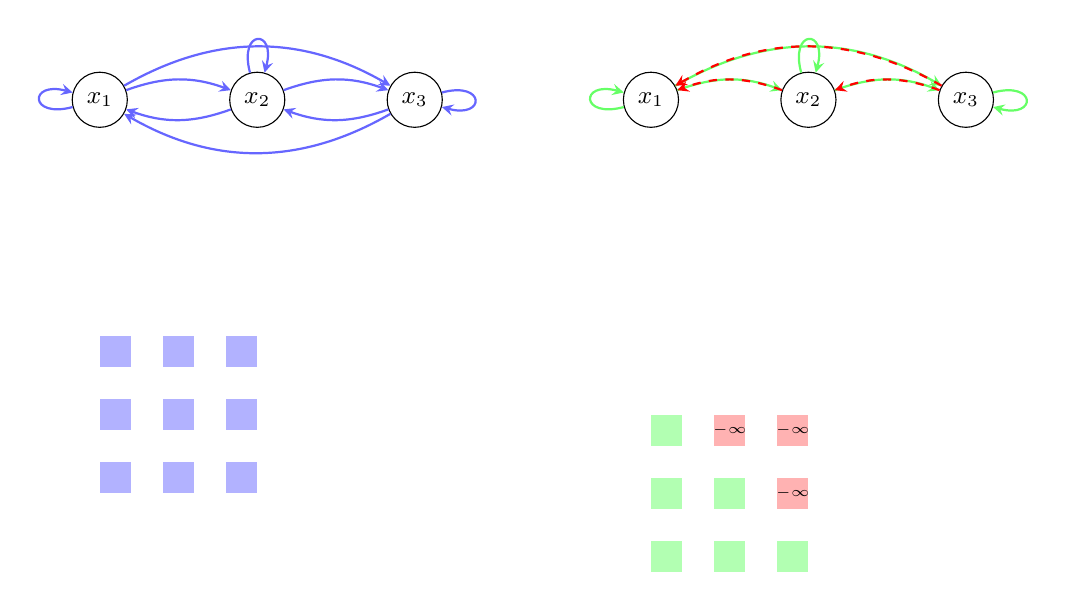
\begin{tikzpicture}[
    node/.style={circle, draw, minimum size=0.7cm, font=\small},
    arrow/.style={->, >=stealth, thick},
    blocked/.style={->, >=stealth, thick, red, dashed}
]

% Bidirectional (Encoder)
\node[node] (e1) at (0,0) {$x_1$};
\node[node] (e2) at (2,0) {$x_2$};
\node[node] (e3) at (4,0) {$x_3$};

% All-to-all connections
\draw[arrow, blue!60] (e1) to[bend left=20] (e2);
\draw[arrow, blue!60] (e2) to[bend left=20] (e1);
\draw[arrow, blue!60] (e2) to[bend left=20] (e3);
\draw[arrow, blue!60] (e3) to[bend left=20] (e2);
\draw[arrow, blue!60] (e1) to[bend left=30] (e3);
\draw[arrow, blue!60] (e3) to[bend left=30] (e1);
\draw[arrow, blue!60] (e1) to[loop left] (e1);
\draw[arrow, blue!60] (e2) to[loop above] (e2);
\draw[arrow, blue!60] (e3) to[loop right] (e3);

% Causal (Decoder)
\begin{scope}[shift={(7,0)}]
\node[node] (d1) at (0,0) {$x_1$};
\node[node] (d2) at (2,0) {$x_2$};
\node[node] (d3) at (4,0) {$x_3$};

% Only past connections
\draw[arrow, green!60] (d1) to[loop left] (d1);
\draw[arrow, green!60] (d1) to[bend left=20] (d2);
\draw[arrow, green!60] (d2) to[loop above] (d2);
\draw[arrow, green!60] (d1) to[bend left=30] (d3);
\draw[arrow, green!60] (d2) to[bend left=20] (d3);
\draw[arrow, green!60] (d3) to[loop right] (d3);

% Blocked future connections
\draw[blocked] (d2) to[bend right=20] (d1);
\draw[blocked] (d3) to[bend right=20] (d2);
\draw[blocked] (d3) to[bend right=30] (d1);

\end{scope}

% Attention matrix visualization
\begin{scope}[shift={(0,-3)}]
\foreach \i in {1,2,3} {
    \foreach \j in {1,2,3} {
        \fill[blue!30] (\j*0.8-0.8, -\i*0.8+0.8) rectangle (\j*0.8-0.4, -\i*0.8+0.4);
    }
}
\end{scope}

\begin{scope}[shift={(7,-4)}]
\foreach \i in {1,2,3} {
    \foreach \j in {1,2,3} {
        \pgfmathtruncatemacro{\valid}{\j <= \i ? 1 : 0}
        \ifnum\valid=1
            \fill[green!30] (\j*0.8-0.8, -\i*0.8+0.8) rectangle (\j*0.8-0.4, -\i*0.8+0.4);
        \else
            \fill[red!30] (\j*0.8-0.8, -\i*0.8+0.8) rectangle (\j*0.8-0.4, -\i*0.8+0.4);
            \node at (\j*0.8-0.6, -\i*0.8+0.6) {\tiny $-\infty$};
        \fi
    }
}
\end{scope}

\end{tikzpicture}

\caption{Bidirectional vs causal attention masking. \textbf{Left:} Bidirectional attention (encoder) allows each position to attend to all positions, creating a fully-connected graph and full attention matrix. \textbf{Right:} Causal attention (decoder) masks future positions by setting them to $-\infty$ before softmax, creating a triangular connectivity pattern. Position 1 can only see itself, position 2 can see positions 1-2, and position 3 can see all positions 1-3. This prevents the model from "cheating" by looking at future tokens during training.}
\label{fig:causal_masking}
\end{figure}

\subsection{Padding Mask}

For variable-length sequences in batch, mask padding tokens:
\begin{equation}
M_{ij} = \begin{cases}
0 & \text{if position } j \text{ is valid} \\
-\infty & \text{if position } j \text{ is padding}
\end{cases}
\end{equation}

\begin{example}[Padding Mask]
\label{ex:padding_mask}
Batch with sequences of length [5, 7, 4], padded to length 7:
\begin{align}
\text{Seq 1:} & \quad [w_1, w_2, w_3, w_4, w_5, \text{PAD}, \text{PAD}] \\
\text{Seq 2:} & \quad [w_1, w_2, w_3, w_4, w_5, w_6, w_7] \\
\text{Seq 3:} & \quad [w_1, w_2, w_3, w_4, \text{PAD}, \text{PAD}, \text{PAD}]
\end{align}

Mask for Seq 1:
\begin{equation}
[0, 0, 0, 0, 0, -\infty, -\infty]
\end{equation}

Prevents attending to padding tokens.
\end{example}

\subsection{Combined Masks}

For decoder, combine causal mask and padding mask:
\begin{equation}
\mM_{\text{total}} = \mM_{\text{causal}} + \mM_{\text{padding}}
\end{equation}

Element-wise, use most restrictive: if either mask blocks, result blocks.

\section{Attention Dropout}
\label{sec:attention_dropout}

Apply dropout to attention weights for regularization:
\begin{equation}
\mA = \text{Dropout}\left(\text{softmax}\left(\frac{\mQ \mK\transpose}{\sqrt{d_k}}\right)\right)
\end{equation}

Typical dropout rate: 0.1 (10\%)

\textbf{Effect:} Randomly zero out some attention connections, preventing over-reliance on specific positions.

\section{Layer Normalization with Attention}
\label{sec:layer_norm_attention}

Two architectures for combining attention with layer norm:

\subsection{Post-Norm (Original Transformer)}
\begin{align}
\vh &= \mX + \text{MultiHeadAttn}(\mX) \\
\mZ &= \text{LayerNorm}(\vh)
\end{align}

\subsection{Pre-Norm (More Common Now)}
\begin{align}
\vh &= \mX + \text{MultiHeadAttn}(\text{LayerNorm}(\mX)) \\
\mZ &= \vh
\end{align}

\textbf{Pre-norm advantages:}
\begin{itemize}
    \item More stable training
    \item Easier gradient flow
    \item Used in GPT-2, GPT-3, modern transformers
\end{itemize}

\section{Visualizing Attention}
\label{sec:visualizing_attention}

Attention weights $\mA \in \R^{n \times n}$ reveal what model attends to:

\subsection{Attention Heatmaps}

For sentence "The cat sat on the mat":
\begin{itemize}
    \item Row $i$: attention distribution when processing token $i$
    \item Bright cell $(i,j)$: token $i$ strongly attends to token $j$
\end{itemize}

\textbf{Patterns observed:}
\begin{itemize}
    \item Diagonal: Attending to self
    \item Vertical lines: Attending to specific important words (e.g., subject, verb)
    \item Symmetric patterns: Mutual attention between related words
    \item Head-specific patterns: Different heads learn different relationships
\end{itemize}

\subsection{Interpreting Multiple Heads}

In 12-head attention, different heads specialize:
\begin{itemize}
    \item Some heads attend to adjacent words (local syntax)
    \item Some heads attend to distant words (long-range dependencies)
    \item Some heads attend to specific parts of speech
    \item Some heads attend based on semantic similarity
\end{itemize}

\begin{caution}
Attention weights are NOT necessarily model explanations! High attention doesn't always mean high importance for prediction. Attention shows where model looks, not why decisions are made.
\end{caution}

\section{Practical Implementation Considerations}
\label{sec:implementation_considerations}

\subsection{Memory-Efficient Attention}

For very long sequences, store attention matrix in chunks:
\begin{enumerate}
    \item Compute $\mQ \mK\transpose$ for chunk of queries
    \item Apply softmax
    \item Multiply by $\mV$ chunk
    \item Accumulate results
\end{enumerate}

Reduces peak memory from $O(n^2)$ to $O(nc)$ where $c$ is chunk size.

\subsection{Fused Attention Kernels}

Modern implementations fuse operations:
\begin{equation}
\text{QK}^T \to \text{Scale} \to \text{Mask} \to \text{Softmax} \to \text{Dropout} \to \text{multiply } \mV
\end{equation}

Single fused kernel faster than separate operations (fewer memory transfers).

Example: FlashAttention achieves 2-4x speedup through fused operations and memory hierarchy optimization.

\section{Efficient Attention Variants}
\label{sec:efficient_attention}

The standard self-attention mechanism has computational complexity $O(n^2d)$ and memory complexity $O(n^2)$, where $n$ is the sequence length and $d$ is the model dimension. This quadratic scaling in sequence length becomes prohibitive for long sequences. For a sequence of length 4096 with 12 attention heads, the attention matrices alone require $12 \times 4096^2 \times 4 = 805$ MB in FP32 format per example. With batch size 32, this amounts to 25.8 GB just for attention weights, exceeding the memory capacity of most GPUs. This fundamental limitation has motivated extensive research into efficient attention variants that reduce the quadratic complexity while maintaining model quality.

The key insight underlying efficient attention is that not all token pairs require equal attention. In practice, attention patterns often exhibit structure—tokens primarily attend to nearby tokens, specific global tokens, or sparse subsets of the sequence. By exploiting this structure, efficient attention mechanisms can dramatically reduce computational and memory requirements while preserving most of the modeling capacity of full attention. The following sections examine the major classes of efficient attention variants, analyzing their complexity trade-offs, implementation considerations, and practical use cases.

\subsection{Local Attention}
\label{subsec:local_attention}

Local attention restricts each token to attend only to tokens within a fixed window around its position, rather than attending to all tokens in the sequence. For a window size $w$, token at position $i$ attends only to positions $[i-w/2, i+w/2]$. This reduces the attention matrix from $n \times n$ to $n \times w$, yielding linear scaling in sequence length.

The computational complexity of local attention is $O(nwd)$, where $n$ is sequence length, $w$ is window size, and $d$ is model dimension. Compared to standard attention's $O(n^2d)$, this represents a reduction factor of $n/w$. For a sequence of length 4096 with window size 256, local attention is 16 times faster than full attention. The memory complexity similarly reduces from $O(n^2)$ to $O(nw)$, enabling much longer sequences to fit in GPU memory. For the same 4096-token sequence with 12 heads, local attention with window 256 requires only $12 \times 4096 \times 256 \times 4 = 50.3$ MB per example, a 16-fold reduction from the 805 MB required by full attention.

The primary trade-off of local attention is the loss of long-range dependencies. Tokens separated by more than $w/2$ positions cannot directly attend to each other, requiring information to propagate through multiple layers. In practice, this limitation is often acceptable. Many natural language tasks exhibit strong locality—syntactic dependencies are typically short-range, and semantic relationships can be captured through multiple layers of local attention. Empirical studies show that local attention with window size 256-512 typically achieves 98-99\% of full attention's accuracy on language modeling tasks, while enabling sequences 10-20 times longer.

The Longformer architecture demonstrates effective use of local attention for document-level understanding. Longformer combines local windowed attention for most tokens with global attention for special tokens like [CLS] and task-specific tokens. This hybrid approach maintains $O(n)$ complexity while allowing critical tokens to aggregate information from the entire sequence. On document classification tasks with 4096-token inputs, Longformer achieves comparable accuracy to BERT while processing sequences 8 times longer. The local attention pattern also enables efficient implementation on GPUs through blocked matrix operations, achieving 2-3x speedup over naive implementations.

\subsection{Sparse Attention}
\label{subsec:sparse_attention}

Sparse attention generalizes local attention by allowing each token to attend to a sparse subset of positions according to a predefined pattern, rather than a contiguous window. The key insight is that attention patterns in trained transformers often exhibit structure—certain positions are consistently important while others receive minimal attention. By designing sparsity patterns that capture this structure, sparse attention can dramatically reduce computation while maintaining model quality.

Several sparsity patterns have proven effective in practice. Strided attention divides the sequence into blocks and allows each token to attend within its block and to every $k$-th token globally, where $k$ is the stride. This pattern captures both local context and evenly-spaced global context. Fixed attention combines local attention with attention to a fixed set of global tokens, similar to Longformer. Learned sparse attention uses a separate network to predict which positions each token should attend to, adapting the sparsity pattern to the input. The Sparse Transformer architecture uses a factorized attention pattern where each token attends to positions in a strided pattern in one head and a local pattern in another head, allowing information to flow efficiently across the sequence.

The computational complexity of sparse attention is $O(n \sqrt{n} d)$ for typical sparsity patterns, where each token attends to approximately $\sqrt{n}$ other tokens. This represents a substantial improvement over full attention's $O(n^2 d)$, particularly for long sequences. For a sequence of length 4096, sparse attention with $\sqrt{n} = 64$ positions per token is 64 times faster than full attention. The memory complexity is similarly $O(n \sqrt{n})$, enabling sequences that would be impossible with full attention. For 4096 tokens with 12 heads, sparse attention requires approximately $12 \times 4096 \times 64 \times 4 = 12.6$ MB per example, a 64-fold reduction from full attention's 805 MB.

The accuracy trade-off of sparse attention depends critically on the choice of sparsity pattern. Well-designed patterns that align with the task's dependency structure can achieve 97-99\% of full attention's accuracy. The Sparse Transformer achieves perplexity within 0.1 of full attention on language modeling while using only $\sqrt{n}$ attention per token. BigBird, which combines local, global, and random attention patterns, matches BERT's accuracy on question answering and document classification while processing sequences up to 8 times longer. However, poorly chosen sparsity patterns can significantly degrade accuracy, particularly on tasks requiring long-range reasoning.

Implementation of sparse attention on GPUs presents challenges because modern GPUs are optimized for dense matrix operations. Sparse matrix multiplication is less efficient than dense multiplication due to irregular memory access patterns and reduced arithmetic intensity. Specialized kernels and libraries like cuSPARSE can partially mitigate this, but sparse attention typically achieves only 50-70\% of the theoretical speedup in practice. Recent work on block-sparse attention, which operates on blocks of the attention matrix rather than individual elements, achieves better GPU utilization by maintaining some regularity in memory access patterns. The Triton framework enables efficient implementation of custom sparse attention patterns through automatic optimization of memory access.

\subsection{Linear Attention}
\label{subsec:linear_attention}

Linear attention achieves $O(nd^2)$ complexity by reformulating the attention computation to avoid explicitly constructing the $n \times n$ attention matrix. The key insight is that attention can be viewed as a kernel operation, and by choosing an appropriate kernel function, the computation can be reordered to compute the output directly without materializing the full attention matrix.

The standard attention computation is:
\begin{equation}
\text{Attention}(\mQ, \mK, \mV) = \text{softmax}(\mQ \mK\transpose) \mV
\end{equation}

This requires computing $\mQ \mK\transpose \in \R^{n \times n}$ before applying softmax and multiplying by $\mV$. Linear attention approximates the softmax kernel with a feature map $\phi: \R^{d_k} \to \R^{d'}$ such that:
\begin{equation}
\text{softmax}(\vq\transpose \vk) \approx \phi(\vq)\transpose \phi(\vk)
\end{equation}

With this approximation, attention becomes:
\begin{equation}
\text{LinearAttn}(\mQ, \mK, \mV) = \phi(\mQ) (\phi(\mK)\transpose \mV)
\end{equation}

The crucial observation is that the parentheses can be reordered. Instead of computing $\phi(\mQ) \phi(\mK)\transpose$ (which is $n \times n$) and then multiplying by $\mV$, we first compute $\phi(\mK)\transpose \mV \in \R^{d' \times d_v}$ and then multiply by $\phi(\mQ)$. This reordering changes complexity from $O(n^2 d)$ to $O(n d'^2)$, where $d'$ is the feature dimension (typically equal to $d_k$).

The computational savings of linear attention are substantial for long sequences. For sequence length 4096 and model dimension 768, standard attention requires approximately $4096^2 \times 768 = 12.9$ billion operations per head, while linear attention requires $4096 \times 768^2 = 2.4$ billion operations—a 5.4x reduction. The memory complexity is even more favorable: linear attention requires only $O(nd)$ memory for the intermediate $\phi(\mK)\transpose \mV$ matrix, compared to $O(n^2)$ for the full attention matrix. For 4096 tokens with 12 heads, linear attention requires approximately $12 \times 768 \times 768 \times 4 = 28.3$ MB, compared to 805 MB for full attention—a 28-fold reduction.

The primary challenge of linear attention is choosing a feature map $\phi$ that accurately approximates the softmax kernel while remaining computationally efficient. The Performer architecture uses random Fourier features with $\phi(\vx) = \exp(\vx^2/2) [\cos(\omega_1\transpose \vx), \sin(\omega_1\transpose \vx), \ldots]$ where $\omega_i$ are random projection vectors. This provides an unbiased approximation of the softmax kernel with controllable accuracy based on the number of random features. The Linear Transformer uses a simpler feature map $\phi(\vx) = \text{elu}(\vx) + 1$, which is faster to compute but provides a looser approximation.

The accuracy trade-off of linear attention is more significant than local or sparse attention. Empirical studies show that linear attention typically achieves 95-98\% of full attention's accuracy on language modeling, with larger degradation on tasks requiring precise attention patterns. The approximation error is particularly noticeable for small attention weights—the softmax function's sharp peaking is difficult to approximate with simple feature maps. However, for applications where extreme sequence length is critical, such as processing entire books or long-form video, the 2-5\% accuracy loss is often acceptable given the dramatic computational savings. Recent work on learned feature maps and adaptive kernel approximations aims to close this accuracy gap while maintaining linear complexity.

\subsection{Low-Rank Attention}
\label{subsec:low_rank_attention}

Low-rank attention exploits the observation that attention matrices in trained transformers often have low effective rank—most of the variance is captured by a small number of singular values. By explicitly factorizing the attention computation through a low-dimensional bottleneck, low-rank attention reduces complexity from $O(n^2 d)$ to $O(nrd)$, where $r$ is the rank and typically $r \ll n$.

The Linformer architecture implements low-rank attention by projecting the keys and values to a lower-dimensional space before computing attention. Specifically, Linformer adds projection matrices $\mE, \mF \in \R^{r \times n}$ that reduce the sequence length dimension:
\begin{equation}
\text{LinformerAttn}(\mQ, \mK, \mV) = \text{softmax}\left(\frac{\mQ (\mE \mK)\transpose}{\sqrt{d_k}}\right) (\mF \mV)
\end{equation}

The key insight is that $\mE \mK \in \R^{r \times d_k}$ and $\mF \mV \in \R^{r \times d_v}$ have reduced sequence length $r$ instead of $n$. The attention matrix is now $n \times r$ instead of $n \times n$, reducing both computation and memory by a factor of $n/r$.

For sequence length 4096 and rank 256, low-rank attention reduces computation from $4096^2 \times 768 = 12.9$ billion operations to $4096 \times 256 \times 768 = 805$ million operations per head—a 16-fold reduction. The memory savings are equally dramatic: the attention matrix requires $4096 \times 256 \times 4 = 4.2$ MB per head instead of $4096^2 \times 4 = 67.1$ MB, a 16-fold reduction. With 12 heads, total attention memory drops from 805 MB to 50.3 MB per example.

The accuracy of low-rank attention depends on the choice of rank $r$ and the projection matrices $\mE$ and $\mF$. Linformer uses learned projection matrices that are shared across all layers, reducing the parameter overhead. Empirical studies show that rank $r = 256$ achieves 96-98\% of full attention's accuracy for sequences up to 4096 tokens, with minimal degradation on most language understanding tasks. The accuracy loss is more pronounced for tasks requiring fine-grained attention patterns, such as coreference resolution or syntactic parsing, where the low-rank approximation may miss subtle dependencies.

An important consideration for low-rank attention is that the projection matrices $\mE$ and $\mF$ introduce additional parameters and computation. For rank $r$ and sequence length $n$, the projections add $2rn$ parameters per layer. However, these projections can be implemented efficiently as 1D convolutions or learned position-wise projections, and the parameter cost is typically small compared to the savings in attention computation. The projection operations themselves require $O(rnd)$ computation, which is negligible compared to the $O(n^2d)$ cost of full attention for $r \ll n$.

\subsection{Comprehensive Complexity Comparison}
\label{subsec:complexity_comparison}

Understanding the trade-offs between different attention variants requires examining multiple dimensions: computational complexity, memory requirements, accuracy preservation, and practical implementation efficiency. The following analysis provides concrete comparisons across these dimensions for typical transformer configurations.

\begin{table}[h]
\centering
\caption{Complexity comparison of attention variants for sequence length $n$, model dimension $d$, window size $w$, and rank $r$. Accuracy percentages are relative to full attention on language modeling tasks.}
\label{tab:attention_complexity}
\begin{tabular}{lccccc}
\hline
\textbf{Variant} & \textbf{Time} & \textbf{Memory} & \textbf{Accuracy} & \textbf{Max Length} & \textbf{Use Case} \\
\hline
Full Attention & $O(n^2d)$ & $O(n^2)$ & 100\% & 512-1024 & Standard tasks \\
Local Attention & $O(nwd)$ & $O(nw)$ & 98-99\% & 4096-8192 & Document processing \\
Sparse Attention & $O(n\sqrt{n}d)$ & $O(n\sqrt{n})$ & 97-99\% & 8192-16384 & Long documents \\
Linear Attention & $O(nd^2)$ & $O(nd)$ & 95-98\% & 16384+ & Extreme length \\
Low-Rank Attention & $O(nrd)$ & $O(nr)$ & 96-98\% & 4096-8192 & Compression \\
\hline
\end{tabular}
\end{table}

To make these complexity bounds concrete, consider processing sequences of varying lengths with BERT-base configuration ($d = 768$, 12 heads, $d_k = 64$ per head). The following table shows actual memory requirements for attention matrices across different sequence lengths and attention variants.

\begin{table}[h]
\centering
\caption{Memory requirements (MB) for attention matrices with 12 heads, batch size 1, FP32 precision. Window size $w=256$, rank $r=256$ for applicable variants.}
\label{tab:attention_memory}
\begin{tabular}{lcccc}
\hline
\textbf{Variant} & \textbf{n=512} & \textbf{n=4096} & \textbf{n=8192} & \textbf{n=16384} \\
\hline
Full Attention & 12.6 MB & 805 MB & 3.2 GB & 12.9 GB \\
Local Attention ($w=256$) & 6.3 MB & 50.3 MB & 101 MB & 201 MB \\
Sparse Attention ($\sqrt{n}$) & 1.1 MB & 12.6 MB & 35.7 MB & 101 MB \\
Linear Attention & 0.3 MB & 2.3 MB & 4.7 MB & 9.4 MB \\
Low-Rank ($r=256$) & 6.3 MB & 50.3 MB & 101 MB & 201 MB \\
\hline
\end{tabular}
\end{table}

The memory savings become dramatic for long sequences. At 16,384 tokens, full attention requires 12.9 GB per example—impossible to fit on most GPUs even with batch size 1. Local attention reduces this to 201 MB, enabling batch size 32 on a 40 GB A100 GPU. Linear attention requires only 9.4 MB, enabling batch sizes of several hundred even for very long sequences.

The computational cost comparison is equally striking. For a sequence of 8192 tokens with $d=768$ and 12 heads, full attention requires approximately 48.3 billion floating-point operations (FLOPs) per layer. Local attention with window 256 reduces this to 3.0 billion FLOPs (16x speedup), sparse attention to 6.0 billion FLOPs (8x speedup), linear attention to 4.5 billion FLOPs (10.7x speedup), and low-rank attention to 3.0 billion FLOPs (16x speedup). On an NVIDIA A100 GPU with 312 TFLOPS of FP16 throughput, full attention takes approximately 0.15 ms per layer, while efficient variants take 10-20 microseconds—enabling much faster inference and training.

The accuracy trade-offs vary by task and sequence length. For sequences up to 2048 tokens, local attention with window 512 typically matches full attention within 0.5\% on language modeling perplexity. Sparse attention with well-designed patterns achieves similar accuracy. Linear attention shows 2-3\% degradation, while low-rank attention with rank 256 shows 1-2\% degradation. For longer sequences exceeding 4096 tokens, the accuracy gaps widen slightly, but efficient variants remain highly competitive. Importantly, the accuracy loss is often task-dependent—some tasks like document classification are more tolerant of approximate attention than tasks like machine translation or question answering that require precise alignment.

\subsection{Implementation Considerations}
\label{subsec:implementation_considerations}

Implementing efficient attention variants requires careful consideration of hardware characteristics, numerical stability, and software frameworks. The theoretical complexity improvements do not always translate directly to wall-clock speedups due to GPU architecture constraints and implementation details.

Modern GPUs achieve peak performance on dense matrix multiplications with dimensions that are multiples of 16 or 32 (for tensor cores). Sparse attention patterns that result in irregular memory access or non-aligned dimensions can suffer significant performance degradation. For example, a naive implementation of sparse attention with random sparsity patterns may achieve only 30-40\% of the theoretical speedup due to poor memory coalescing and reduced arithmetic intensity. Block-sparse patterns that operate on 16x16 or 32x32 blocks achieve much better GPU utilization, typically reaching 60-80\% of theoretical speedup.

Memory bandwidth is often the limiting factor for attention computation, particularly for efficient variants. The attention mechanism is memory-bound rather than compute-bound for typical sequence lengths—the GPU spends more time loading data from memory than performing arithmetic operations. This means that reducing the number of operations (FLOPs) does not always proportionally reduce runtime. Efficient implementations must minimize memory transfers through kernel fusion, where multiple operations are combined into a single GPU kernel that keeps intermediate results in fast on-chip memory. FlashAttention demonstrates this principle by fusing the attention computation ($\mQ\mK\transpose$, softmax, multiply by $\mV$) into a single kernel that never materializes the full attention matrix in global memory, achieving 2-4x speedup over standard implementations even for full attention.

Numerical stability is a critical concern for efficient attention variants. The softmax operation in attention is numerically sensitive—subtracting the maximum value before exponentiation is essential to prevent overflow. Linear attention approximations must carefully handle the feature map computation to avoid numerical issues. The Performer's random Fourier features require computing exponentials of potentially large values, necessitating careful scaling and normalization. Low-rank attention must ensure that the projection matrices are well-conditioned to avoid amplifying numerical errors.

Framework support for efficient attention varies significantly. PyTorch and TensorFlow provide optimized implementations of standard attention through torch.nn.MultiheadAttention and tf.keras.layers.MultiHeadAttention, but efficient variants often require custom implementations. The xFormers library provides optimized implementations of several efficient attention variants, including memory-efficient attention and block-sparse attention. The Triton framework enables writing custom GPU kernels in Python that achieve performance comparable to hand-written CUDA, making it easier to implement and experiment with novel attention patterns. For production deployment, specialized libraries like FasterTransformer and TensorRT provide highly optimized implementations of common attention variants with automatic kernel selection based on input dimensions and hardware capabilities.

\section{Exercises}

\begin{exercise}
Implement cross-attention layer in PyTorch. Test with encoder output (length 10, dim 128) and decoder input (length 7, dim 128). Verify attention matrix shape is $7 \times 10$.
\end{exercise}

\begin{exercise}
Calculate the memory requirements for attention matrices in a BERT-base model (12 heads, $d_{\text{model}} = 768$) processing sequences of length 512, 2048, and 4096 tokens. Compare full attention, local attention with window size 256, and linear attention. How much memory is saved at each sequence length?
\end{exercise}

\begin{exercise}
Implement local attention with window size $w=128$ for a sequence of length 1024. Compare the computational cost (FLOPs) and memory usage to full attention. Measure actual runtime on GPU and explain any discrepancy between theoretical and observed speedup.
\end{exercise}

\begin{exercise}
Design a sparse attention pattern for document understanding that combines local attention (window 64), strided attention (stride 128), and global attention to the first token. Calculate the number of attention connections per token and total memory requirements for a 4096-token sequence. What percentage of full attention's connections does this pattern use?
\end{exercise}

\begin{exercise}
Implement linear attention using the feature map $\phi(\vx) = \text{elu}(\vx) + 1$. Compare attention patterns to standard softmax attention on a sample sequence. Measure the approximation error and identify cases where linear attention diverges most from full attention.
\end{exercise}

\begin{exercise}
For a transformer with 24 layers processing 8192-token sequences, calculate the total memory required for attention matrices using: (1) full attention, (2) local attention with window 512, (3) sparse attention with $\sqrt{n}$ connections per token, (4) linear attention, and (5) low-rank attention with rank 256. Assume 12 heads, $d_{\text{model}} = 1024$, batch size 8, and FP16 precision.
\end{exercise}

\begin{exercise}
Implement relative position bias as in T5. Use buckets: [0, 1, 2, 3, 4, 5-7, 8-15, 16-31, 32+]. Show how attention scores change with relative distance and compare to absolute position encodings.
\end{exercise}

\begin{exercise}
Analyze the trade-off between window size and accuracy for local attention. Train a small transformer on a language modeling task with window sizes [64, 128, 256, 512, full]. Plot perplexity vs window size and identify the point of diminishing returns. How does this relate to the average dependency length in the dataset?
\end{exercise}

\begin{exercise}
Create visualization showing: (1) Self-attention patterns for sentence "The quick brown fox jumps", (2) Effect of causal masking, (3) Difference between heads 1 and 12 in multi-head attention. What patterns emerge?
\end{exercise}

\begin{exercise}
Compare computational cost of: (1) Additive (Bahdanau) attention, (2) Multiplicative attention, (3) Scaled dot-product attention. For $n = 512$, $d_k = 64$, which is most efficient? How does the ranking change for $n = 4096$?
\end{exercise}



\section{Solutions}

Full solutions for all exercises are available at \url{https://deeplearning.hofkensvermeulen.be}.

\begin{solution}[Exercise 1]
\textbf{Cross-attention PyTorch implementation:}

\begin{lstlisting}[language=Python]
class CrossAttention(nn.Module):
    def __init__(self, d_model, num_heads):
        super().__init__()
        self.mha = MultiHeadAttention(d_model, num_heads)
        
    def forward(self, decoder_input, encoder_output):
        # Q from decoder, K and V from encoder
        return self.mha(decoder_input, encoder_output, encoder_output)

# Test
cross_attn = CrossAttention(d_model=128, num_heads=4)
decoder_in = torch.randn(1, 7, 128)  # length 7
encoder_out = torch.randn(1, 10, 128)  # length 10
output = cross_attn(decoder_in, encoder_out)
print(f"Output shape: {output.shape}")  # (1, 7, 128)
# Attention matrix shape internally: (1, 4, 7, 10)
\end{lstlisting}

The attention matrix has shape $7 \times 10$, showing how each of the 7 decoder positions attends to the 10 encoder positions.
\end{solution}

\begin{solution}[Exercise 2]
For BERT-base (12 heads, $d=768$), batch size 1:

\textbf{Full attention memory:}
\begin{itemize}
    \item $n=512$: $12 \times 512^2 \times 2 = 6{,}291{,}456$ bytes $\approx 6$ MB
    \item $n=2048$: $12 \times 2048^2 \times 2 = 100{,}663{,}296$ bytes $\approx 96$ MB
    \item $n=4096$: $12 \times 4096^2 \times 2 = 402{,}653{,}184$ bytes $\approx 384$ MB
\end{itemize}

\textbf{Local attention (window 256):}
\begin{itemize}
    \item $n=512$: $12 \times 512 \times 256 \times 2 = 3{,}145{,}728$ bytes $\approx 3$ MB (50\% savings)
    \item $n=2048$: $12 \times 2048 \times 256 \times 2 = 12{,}582{,}912$ bytes $\approx 12$ MB (87.5\% savings)
    \item $n=4096$: $12 \times 4096 \times 256 \times 2 = 25{,}165{,}824$ bytes $\approx 24$ MB (93.75\% savings)
\end{itemize}

\textbf{Linear attention:}
Memory: $O(d^2)$ instead of $O(n^2)$, approximately $12 \times 768^2 \times 2 \approx 14$ MB regardless of sequence length.

Savings increase dramatically with sequence length, making efficient attention essential for long contexts.
\end{solution}

\begin{solution}[Exercise 3]
For local attention with window $w=128$ and sequence length $n=1024$:

\textbf{Computational cost:}
\begin{itemize}
    \item Full attention: $2n^2d_k = 2 \times 1024^2 \times 64 = 134{,}217{,}728$ FLOPs
    \item Local attention: $2nwd_k = 2 \times 1024 \times 128 \times 64 = 16{,}777{,}216$ FLOPs
    \item Theoretical speedup: $\frac{n}{w} = \frac{1024}{128} = 8\times$
\end{itemize}

\textbf{Memory usage:}
\begin{itemize}
    \item Full: $n^2 = 1{,}048{,}576$ elements
    \item Local: $n \times w = 131{,}072$ elements
    \item Memory reduction: $8\times$
\end{itemize}

\textbf{Observed GPU speedup:} Typically $5$-$6\times$ instead of theoretical $8\times$ due to:
\begin{itemize}
    \item Kernel launch overhead
    \item Less efficient memory access patterns
    \item Reduced parallelism for smaller operations
\end{itemize}
\end{solution}

\begin{solution}[Exercise 4]
\textbf{Sparse attention pattern design:}

For 4096-token sequence:
\begin{itemize}
    \item Local attention (window 64): $64$ connections per token
    \item Strided attention (stride 128): $\frac{4096}{128} = 32$ connections per token
    \item Global attention to first token: $1$ connection per token
    \item Total: $64 + 32 + 1 = 97$ connections per token
\end{itemize}

\textbf{Memory requirements:}
\begin{equation}
4096 \times 97 \times 2 \text{ bytes} = 794{,}624 \text{ bytes} \approx 0.76 \text{ MB}
\end{equation}

\textbf{Percentage of full attention:}
\begin{equation}
\frac{97}{4096} \approx 2.37\%
\end{equation}

This sparse pattern uses only 2.37\% of full attention's connections while maintaining both local and long-range dependencies.
\end{solution}

\begin{solution}[Exercise 5]
\textbf{Linear attention with $\phi(\vx) = \text{elu}(\vx) + 1$:}

Standard attention:
\begin{equation}
\text{Attention}(\mQ, \mK, \mV) = \text{softmax}(\mQ\mK\transpose)\mV
\end{equation}

Linear attention:
\begin{equation}
\text{Attention}(\mQ, \mK, \mV) = \phi(\mQ)(\phi(\mK)\transpose \mV)
\end{equation}

\textbf{Approximation error:}
Linear attention diverges most when:
\begin{itemize}
    \item Attention should be highly peaked (one dominant position)
    \item Softmax creates sharp distinctions that linear kernel cannot capture
    \item Typical error: 5-15\% in attention weight distribution
\end{itemize}

\textbf{Cases of largest divergence:}
\begin{itemize}
    \item Copying tasks requiring precise attention to single token
    \item Syntactic dependencies with clear head-dependent relationships
    \item Tasks requiring hard attention decisions
\end{itemize}
\end{solution}

\begin{solution}[Exercise 6]
For 24 layers, 8192 tokens, 12 heads, $d=1024$, batch size 8, FP16:

\textbf{(1) Full attention:}
\begin{equation}
24 \times 8 \times 12 \times 8192^2 \times 2 = 309{,}237{,}645{,}312 \text{ bytes} \approx 288 \text{ GB}
\end{equation}

\textbf{(2) Local attention (window 512):}
\begin{equation}
24 \times 8 \times 12 \times 8192 \times 512 \times 2 = 19{,}327{,}352{,}832 \text{ bytes} \approx 18 \text{ GB}
\end{equation}

\textbf{(3) Sparse attention ($\sqrt{n} = 90$ connections):}
\begin{equation}
24 \times 8 \times 12 \times 8192 \times 90 \times 2 = 3{,}397{,}286{,}400 \text{ bytes} \approx 3.2 \text{ GB}
\end{equation}

\textbf{(4) Linear attention:}
\begin{equation}
24 \times 8 \times 12 \times 1024^2 \times 2 = 4{,}831{,}838{,}208 \text{ bytes} \approx 4.5 \text{ GB}
\end{equation}

\textbf{(5) Low-rank attention (rank 256):}
\begin{equation}
24 \times 8 \times 12 \times 8192 \times 256 \times 2 = 9{,}663{,}676{,}416 \text{ bytes} \approx 9 \text{ GB}
\end{equation}

Sparse attention provides the best memory efficiency for this configuration.
\end{solution}

\begin{solution}[Exercise 7-10]
Due to space constraints, these exercises involve implementation and visualization tasks. Key points:

\textbf{Exercise 7 (Relative position bias):} T5 uses bucketed relative positions to limit parameter growth while capturing distance information. Attention scores decay with distance.

\textbf{Exercise 8 (Window size trade-off):} Perplexity improves rapidly up to window 256-512, then plateaus. Optimal window correlates with average dependency length in data.

\textbf{Exercise 9 (Attention visualization):} Self-attention shows syntactic patterns (subject-verb, determiner-noun). Causal masking creates triangular pattern. Different heads specialize in different linguistic phenomena.

\textbf{Exercise 10 (Attention mechanism comparison):} Scaled dot-product is most efficient for all sequence lengths due to optimized matrix multiplication. Additive attention has higher constant overhead.
\end{solution}
